%Copyright 2019 Christopher M. Jermaine (cmj4@rice.edu) and Risa B. Myers (rbm2@rice.edu)
%
%Licensed under the Apache License, Version 2.0 (the "License");
%you may not use this file except in compliance with the License.
%You may obtain a copy of the License at
%
%    https://www.apache.org/licenses/LICENSE-2.0
%
%Unless required by applicable law or agreed to in writing, software
%distributed under the License is distributed on an "AS IS" BASIS,
%WITHOUT WARRANTIES OR CONDITIONS OF ANY KIND, either express or implied.
%See the License for the specific language governing permissions and
%limitations under the License.
%===============================================================
\documentclass[aspectratio=169]{beamer}
\mode<presentation> 
{
\usetheme[noshadow, minimal,numbers,riceb,nonav]{Rice}
\usefonttheme[onlymath]{serif}
\setbeamercovered{transparent}
}
\useinnertheme{rectangles}

\usepackage[english]{babel}

\usepackage{mathptmx}
\usepackage{helvet}
\usepackage{courier}
\usepackage[T1]{fontenc}
\usepackage{trajan}
\usepackage{ textcomp }
\usepackage{listings}

\newenvironment{noindentitemize}
{ \begin{itemize}
 \setlength{\itemsep}{1.5ex}
  \setlength{\parsep}{0pt}   
  \setlength{\parskip}{0pt}
 \addtolength{\leftskip}{-2em}
 }
{ \end{itemize} }

\newenvironment{noindentitemize2}
{ \begin{itemize}
  \setlength{\itemsep}{0ex}
  \setlength{\parskip}{0pt}
  \setlength{\parsep}{0pt}   
  \addtolength{\leftskip}{-2em}  }
{ \end{itemize} }



\lstnewenvironment{SQL}
  {\lstset{
        aboveskip=5pt,
        belowskip=5pt,
        escapechar=!,
        mathescape=true,
        upquote=true,
        language=SQL,
        basicstyle=\linespread{0.94}\ttfamily\footnotesize,
        morekeywords={PRINT, CURSOR, OPEN, FETCH, CLOSE, DECLARE, BEGIN, END, PROCEDURE, FOR, EACH, WITH, PARTITION, 	TEST, WHETHER, PROBABILITY, OUT,LOOP,IF,CONTINUE, HANDLER,CALL, FUNCTION, RETURNS, LANGUAGE,BODY,RETURN, REPLACE,plpgsql,
        RAISE, NOTICE,
        REPLACE, ROW, BEFORE, EXIT, TEXT, REFCURSOR, QUOTE_LITERAL, DELIMITER,CONCAT,FOUND,LEAVE },
        deletekeywords={VALUE, PRIOR},
        showstringspaces=true}
        \vspace{0pt}%
        \noindent\minipage{0.65\textwidth}}
  {\endminipage\vspace{0pt}}
  
  
\lstnewenvironment{SQLtiny}
  {\lstset{
        aboveskip=5pt,
        belowskip=5pt,
        escapechar=!,
        mathescape=true,
        upquote=true,
        language=SQL,
        basicstyle=\linespread{0.94}\ttfamily\tiny,
        morekeywords={PRINT, CURSOR, OPEN, FETCH, CLOSE, DECLARE, BEGIN, END, PROCEDURE, FOR, EACH, WITH, PARTITION, 	TEST, WHETHER, PROBABILITY, OUT,LOOP,IF,CONTINUE, HANDLER,CALL, FUNCTION, RETURNS, LANGUAGE,BODY,RETURN, REPLACE,plpgsql,
        RAISE, NOTICE,
        REPLACE, ROW, BEFORE, EXIT, TEXT, REFCURSOR, QUOTE_LITERAL, DELIMITER,CONCAT,FOUND,LEAVE },
       deletekeywords={VALUE, PRIOR},
        showstringspaces=true}
        \vspace{0pt}%
        \noindent\minipage{0.47\textwidth}}
  {\endminipage\vspace{0pt}}

%===============================================================%

\title[]
{Tools \& Models for Data Science}

\subtitle{Optimization--Gradient Descent}

\author[]{Chris Jermaine \& Risa Myers}
\institute
{
  Rice University 
}

\date[]{}

\subject{Beamer}


\begin{document}

\begin{frame}
 \titlepage
\end{frame}
%***********************************************************
\begin{frame}{Optimization}

\begin{itemize}
\item At the heart of all ``learning'' frameworks discussed
	\begin{itemize}
	\item Is optimization!
	\end{itemize}
\item Why?
	\begin{itemize}
	\item Well, it's explicit in case of loss functions, MLE
	\item Implicitly in case of Bayesian
	\end{itemize}
\item Means we need to ask: how to solve optimization problems?
	\begin{itemize}
	\item Fundamental question in data science!!
	\end{itemize}
\end{itemize}

\end{frame}
%***********************************************************
\begin{frame}{Desired Properties}

\begin{itemize}
\item To be useful for data science, an optimization framework should be
\begin{itemize}
	\item Easily applied to many types of optimization problems
	\item Scalable (easily built in Spark, for example)
	\item Fast (quick convergence)
\end{itemize}
\end{itemize}

\end{frame}
%***********************************************************
\begin{frame}{Most Widely Used Optimization Framework Is...}

\begin{itemize}
\item For (big) data science, at least...
	\begin{itemize}
	\item Gradient descent!
	\end{itemize}
\item What's the idea?
	\begin{itemize}
	\item GD is an iterative algorithm
	\item Goal: choose $\Theta^*$ to minimize/maximize the Loss function $L (\Theta)$
	\item Tries to incrementally improve current solution
	\item At step $i$, $\Theta_i$ is current guess for $\Theta^*$
	\end{itemize}
\end{itemize}

\end{frame}
%***********************************************************
\begin{frame}{Gradient Descent Intuition}

\begin{columns}[T]
\begin{column}{0.5\textwidth}
\begin{itemize}
\item Look at the slope of L
\item Go in the direction of steepest descent
\item Don't go too far!
\item Stop when your parameter values aren't changing much
\item Can end up oscillating if your step size is too big
\end{itemize}
\end{column}
\begin{column}{0.5\textwidth}
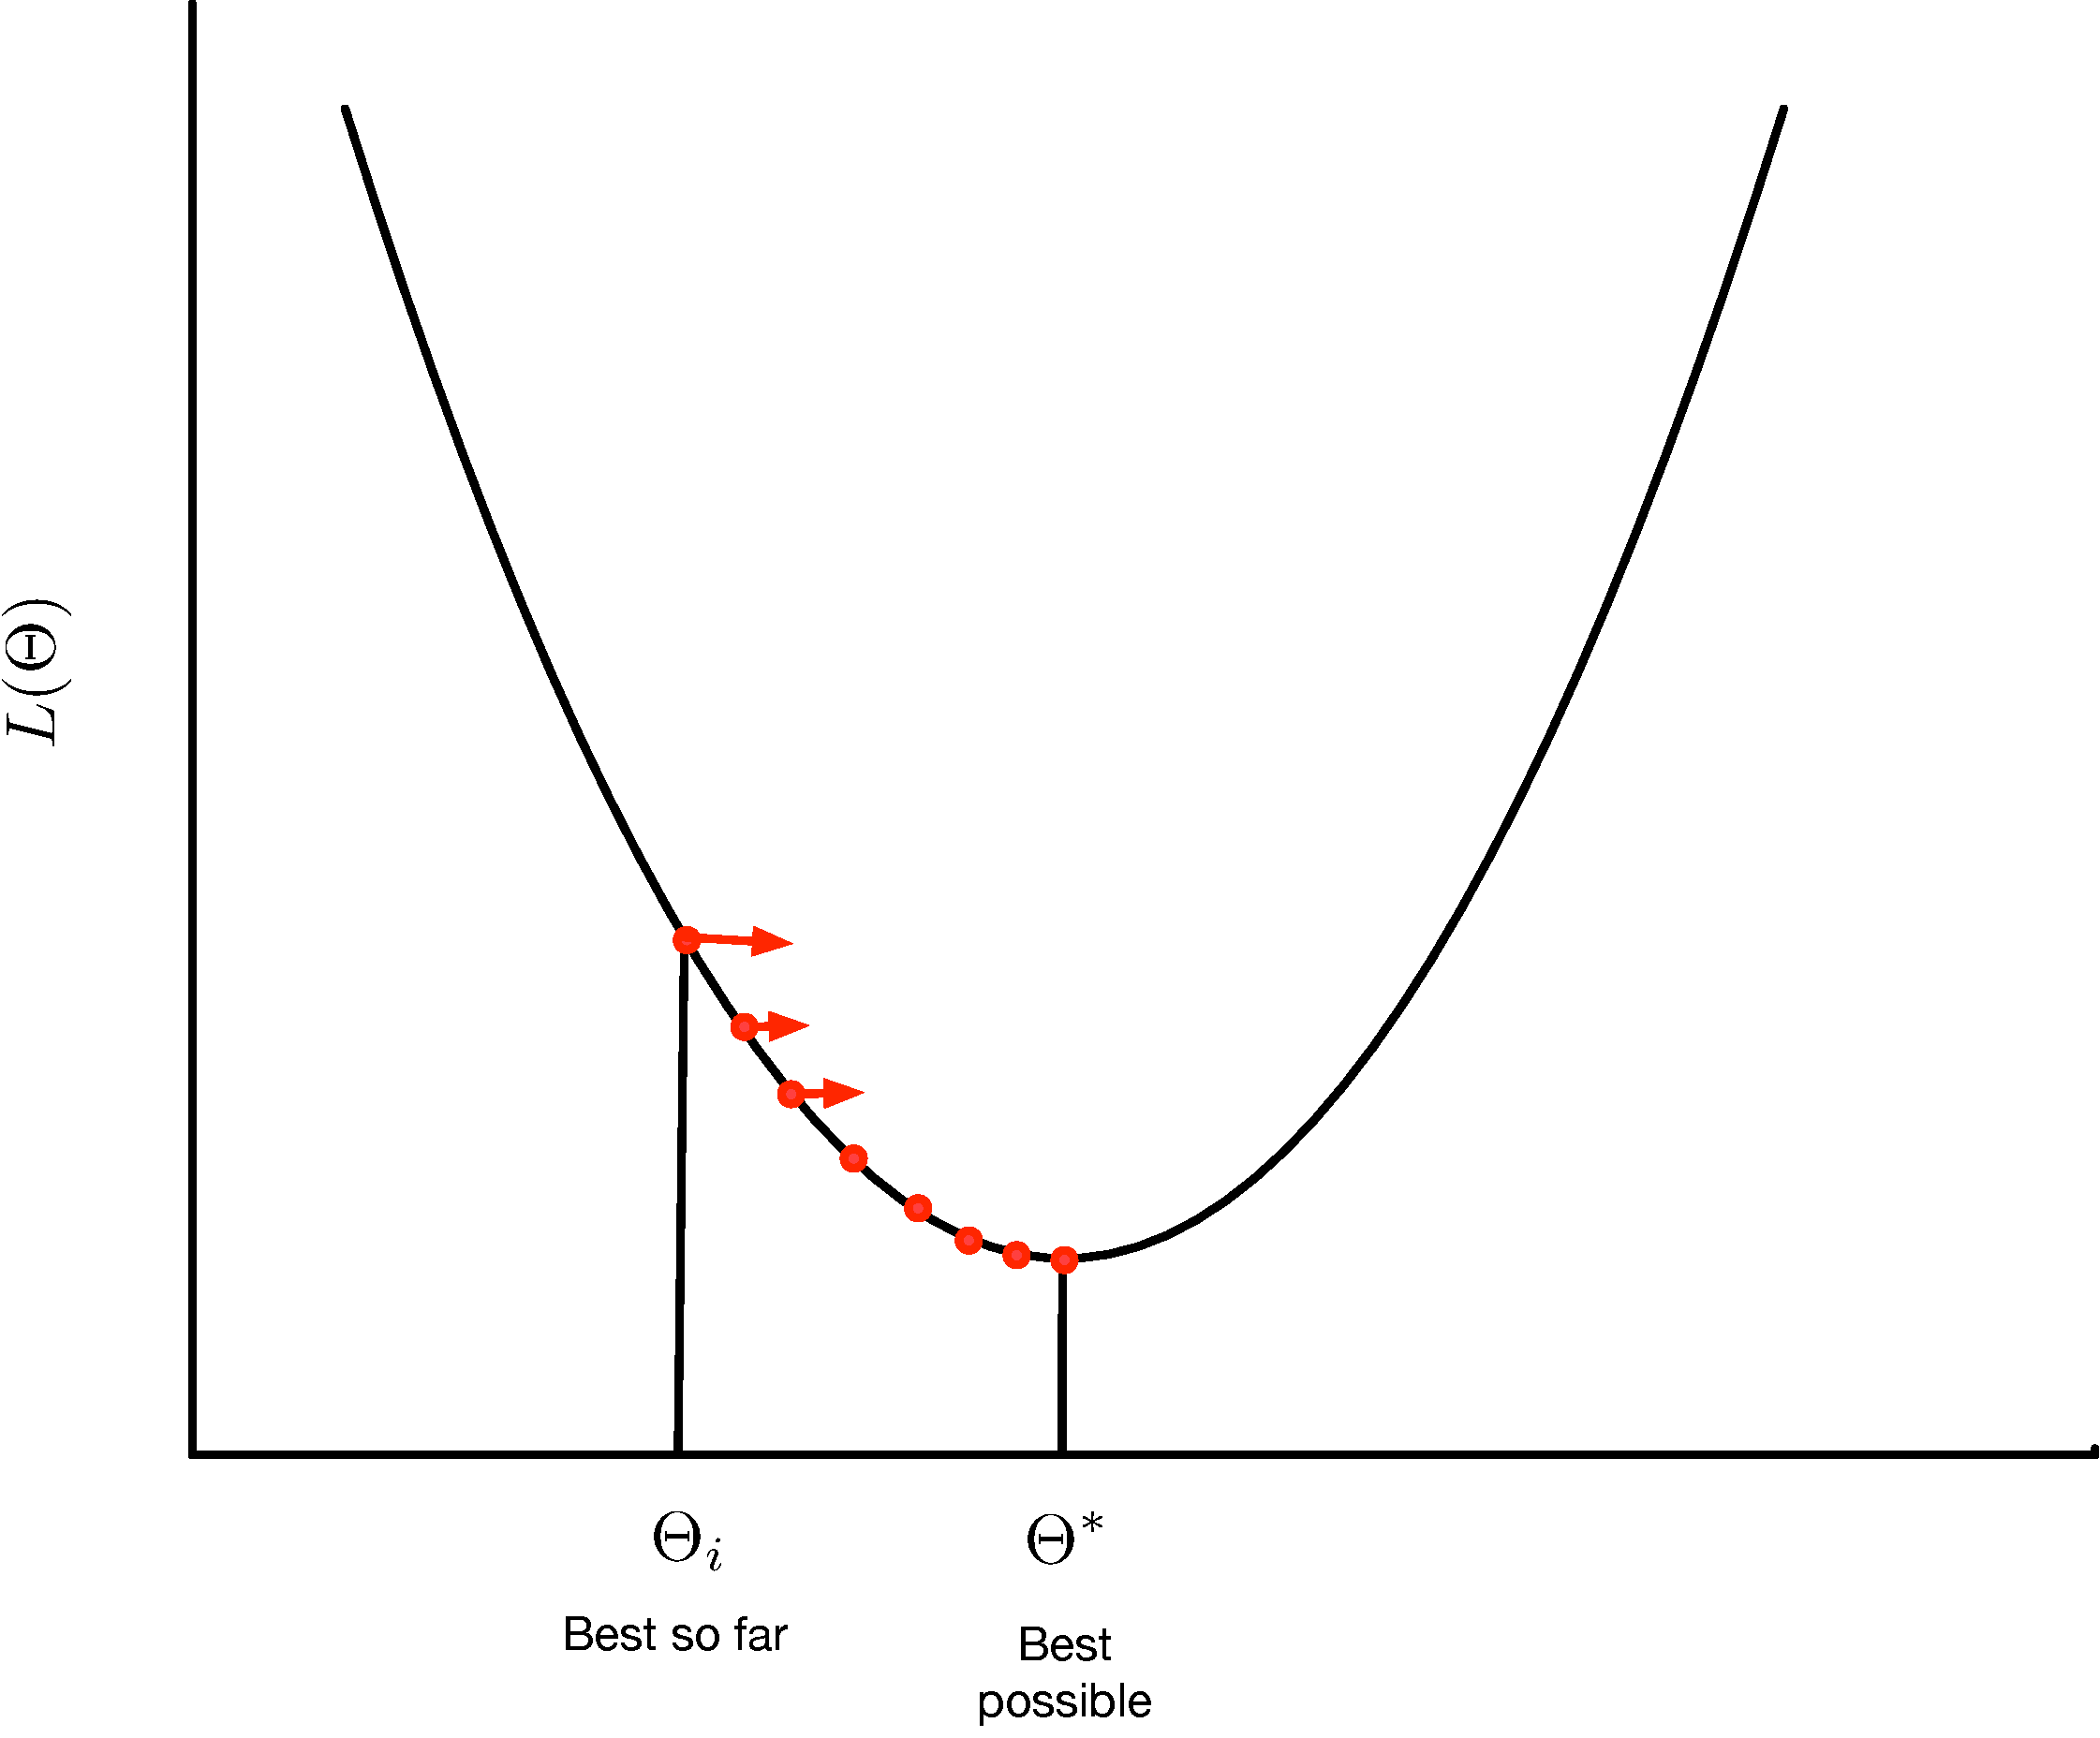
\includegraphics[width=1\textwidth]{lectGD/gd1V2.pdf}
\end{column}
\end{columns}

\end{frame}
%***********************************************************
\begin{frame}[fragile]{Gradient Descent}

\begin{columns}[T]
\begin{column}{0.3\textwidth}
\begin{noindentitemize}
\item Basic algorithm:
\end{noindentitemize}
\begin{SQL}
$\Theta_1 \leftarrow \textrm{non-stupid guess for } \Theta^*$;
$i \leftarrow 1$;
repeat {
  $\Theta_{i + 1} \leftarrow \Theta_{i} - \lambda \nabla L (\Theta_{i})$;
  $i \leftarrow i + 1$;
} while ($||\Theta_{i} - \Theta_{i - 1}||_1 > \epsilon$)
\end{SQL} 
\end{column}
\begin{column}{0.7\textwidth}
\begin{itemize}
\vspace{3em}
\item  $\lambda \nabla L (\Theta_{i})$ is some distance along the direction of steepest descent
\item $||\Theta_{i} - \Theta_{i - 1}||_1$ is the L$_1$ distance, the absolute value of the change in parameter value(s)
\end{itemize}
\end{column}
\end{columns}

\end{frame}
%***********************************************************
\begin{frame}[fragile]{Gradient Descent}

\begin{noindentitemize}
\item Basic algorithm:
\end{noindentitemize}

\begin{SQL}
$\Theta_1 \leftarrow \textrm{non-stupid guess for } \Theta^*$;
$i \leftarrow 1$;
repeat {
  $\Theta_{i + 1} \leftarrow \Theta_{i} - \lambda \nabla L (\Theta_{i})$;
  $i \leftarrow i + 1$;
} while ($||\Theta_{i} - \Theta_{i - 1}||_1 > \epsilon$)
\end{SQL} 

\begin{itemize}
\item $\lambda$ is the ``learning rate''
\begin{itemize}
\item how far you go a each step in the direction of steepest descent
\item Controls speed of convergence
\item If too big, algorithm will oscillate
\item If too small, algorithm will take a very long time to run
\end{itemize}
\item $\nabla L (\Theta_{i})$ is the gradient of $L$ evaluated at $\Theta_{i}$
\end{itemize}

\end{frame}
%***********************************************************
\begin{frame}[fragile]{Stopping Condition}

\begin{noindentitemize}
\item Here we use 
\end{noindentitemize}
\begin{SQL}
while ($||\Theta_{i} - \Theta_{i - 1}||_1 > \epsilon$)
\end{SQL}
\begin{itemize}
\item Easy to compute
\item Efficient because it just requires checking for small changes in \textbf{model}
\item Serves as a \textbf{proxy} for the change in the \textbf{loss function}
\item But does not always make sense (big change in model can mean small change in accuracy)
\end{itemize}

\end{frame}
%***********************************************************
\begin{frame}[fragile]{Stopping Condition}

\begin{itemize}
\item If feasible, instead use
\end{itemize}
\begin{SQL}
while (|$L(\Theta_{i}) - L(\Theta_{i - 1})| > \epsilon$)
\end{SQL}
\begin{itemize}
\item Drawback: requires loss computation... can be expensive
\item Can be more expensive than another iteration
\item Alternative: Stochastic Gradient Descent or Minibatch % stochastic - just 1 data point; minibatch - small # of data points
\begin{itemize}
\item Use a small sample of the dataset
\item Note: the parameters ($\Theta$) will never stop changing, due to different data points used each time
\item Much more difficult to decide when to stop
\end{itemize}
\end{itemize}

\end{frame}
%***********************************************************

\begin{frame}{A Gradient}

\begin{itemize}
\item What's a ``gradient''?
\item Gradient is the multi-dimensional analog to a derivative
	\begin{itemize}
	\item If $L(.)$ accepts a vector
	\item $\nabla L$ is a vector-valued function 
	\begin{itemize}
	\item That is, accepts a vector $\Theta$
	\item Returns a vector, $\Theta'$
	\item whose $i$th entry is $i$th partial derivative evaluated at $\Theta$
\end{itemize}
	\end{itemize}
\end{itemize}

\end{frame}
%***********************************************************
\begin{frame}{Example}

\begin{columns}[T]
\begin{column}{0.5\textwidth}
\begin{itemize}
\item Returning to linear regression...
	\begin{itemize}
	\item Want a line to fit points $\langle 118, 122, 145, 149, 186 \rangle$ 
	\item At time ticks 
		$t$ in $\langle 1, 2, 3, 4, 5 \rangle$
	\item Prediction $f(t | b, m) = b + m \times t$
	\item Loss $L(b, m) = \sum_i \left(f(t_i | b, m) - x_i \right)^2$
	\item Model parameters: \{b,m\}  \{intercept, slope\} %y = 16.3x + 95.1    R² = 0.9006
	\item Use L$_2$ loss: Least Squares
	\end{itemize}
\end{itemize}
\end{column}
\begin{column}{0.5\textwidth}
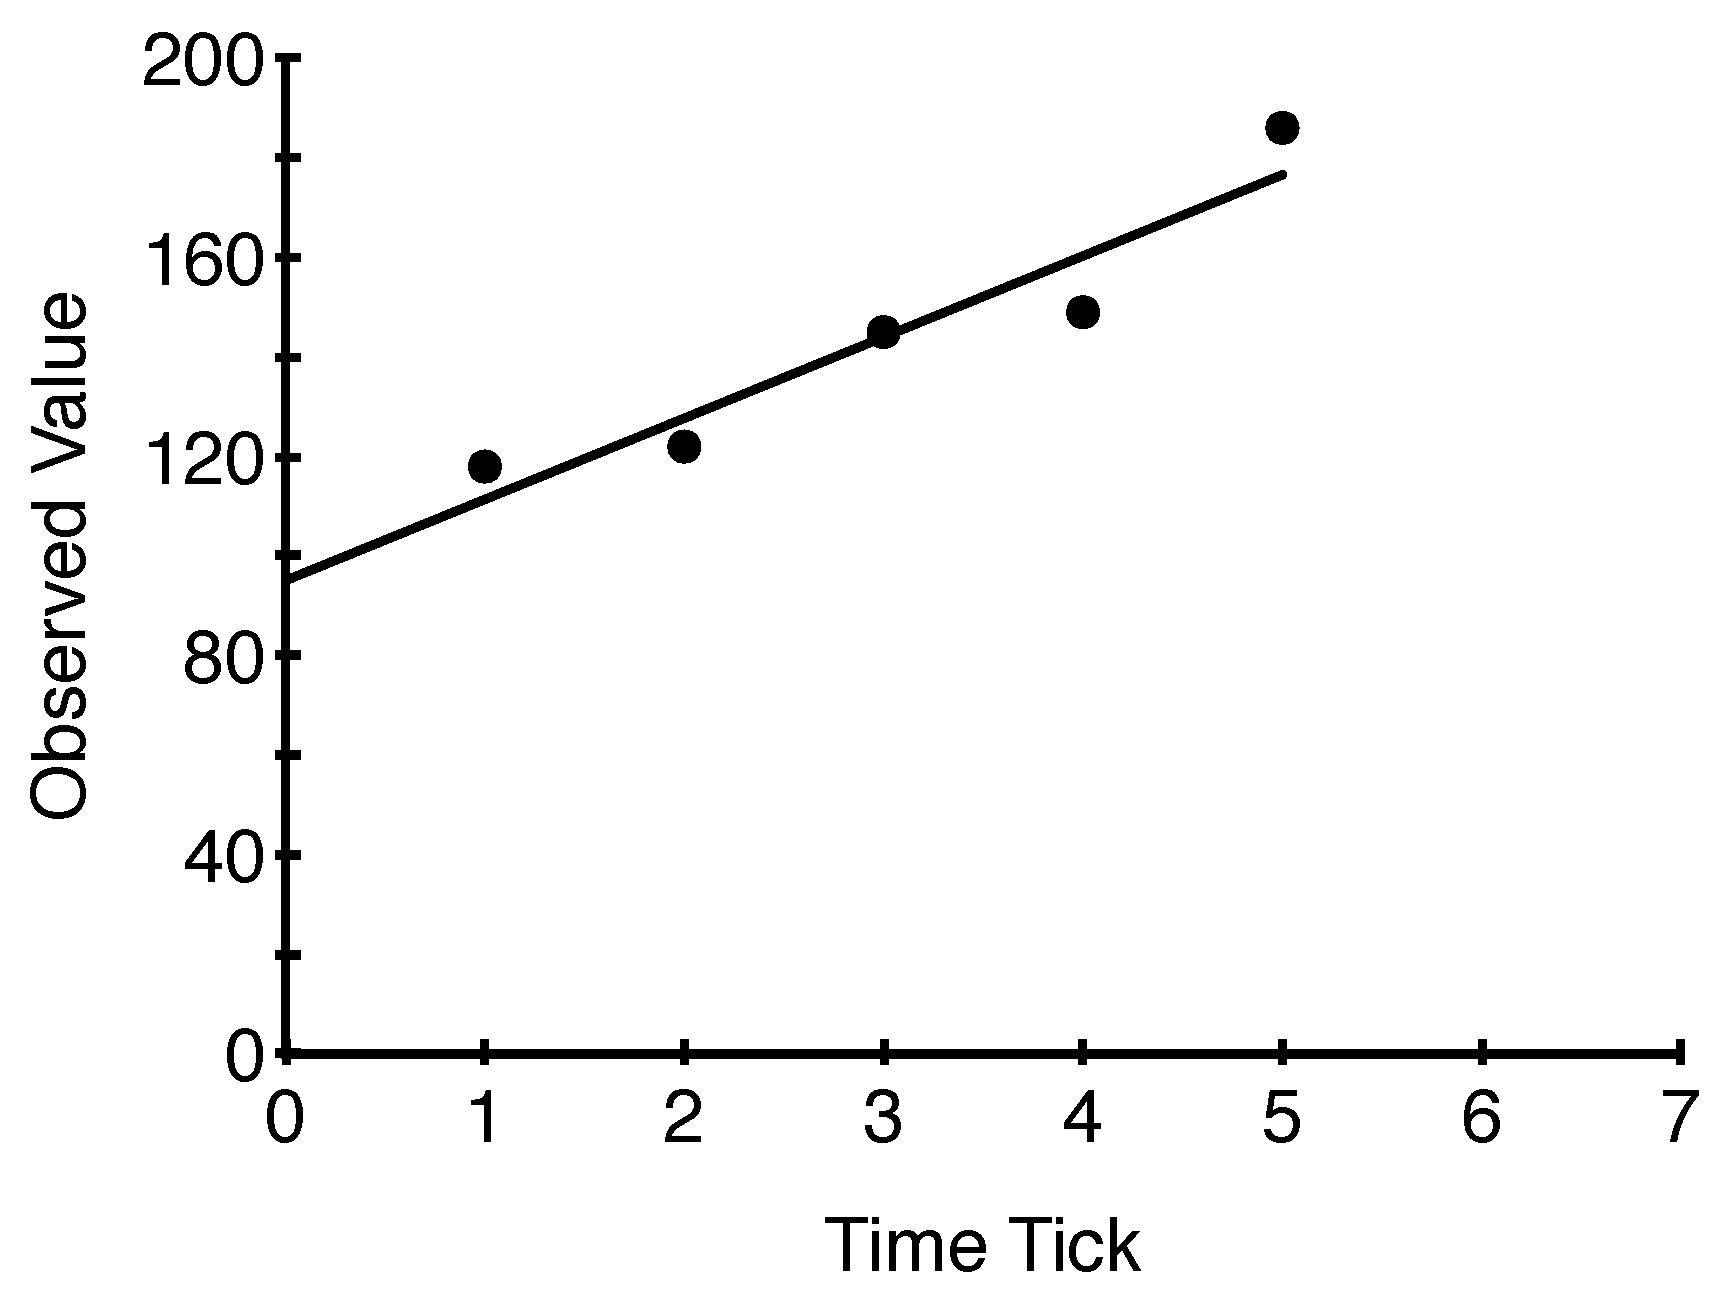
\includegraphics[width=1\textwidth]{lectGD/gdLR1fit.pdf}
\end{column}
\end{columns}

\end{frame}

%***********************************************************
\begin{frame}{Gradient Descent and Big Data}

\begin{itemize}
\item So $\nabla L(b, m) = $
        $$ \langle \sum_i 2(f(t_i | b, m) - x_i), \sum_i 2t_i(f(t_i | b, m) - x_i) \rangle$$
\item Derivation is left as an exercise to the user (or look at the last slide in the deck)
\item Gradient of this form (summing up values over all the data points) is very common
\item[?] Why is this so good for ``big data'', MapReduce/Spark?
\end{itemize}

\end{frame}

%***********************************************************
\begin{frame}{Gradient Descent and Big Data}

\begin{itemize}
\item So $\nabla L(b, m) = $
        $$ \langle \sum_i 2(f(t_i | b, m) - x_i), \sum_i 2t_i(f(t_i | b, m) - x_i) \rangle$$
\item Gradient of this form (summing up values over all the data points) is very common
\item Why is this so good for ``big data'', MapReduce/Spark?
\begin{itemize}
\item Sums are easily parallelized
\end{itemize}
\end{itemize}

\end{frame}
%***********************************************************
\begin{frame}[fragile]{What do Gradient Descent Steps Look Like?}

\begin{columns}[c]
\begin{column}{0.4\textwidth}

\begin{SQL}
$\Theta_1 \leftarrow \textrm{non-stupid guess for } \Theta^*$;
repeat {
 update m
 update b
 } while ($||\Theta_{i} - \Theta_{i - 1}||_1 > \epsilon$)
\end{SQL} 
\end{column}
\begin{column}{0.3\textwidth}
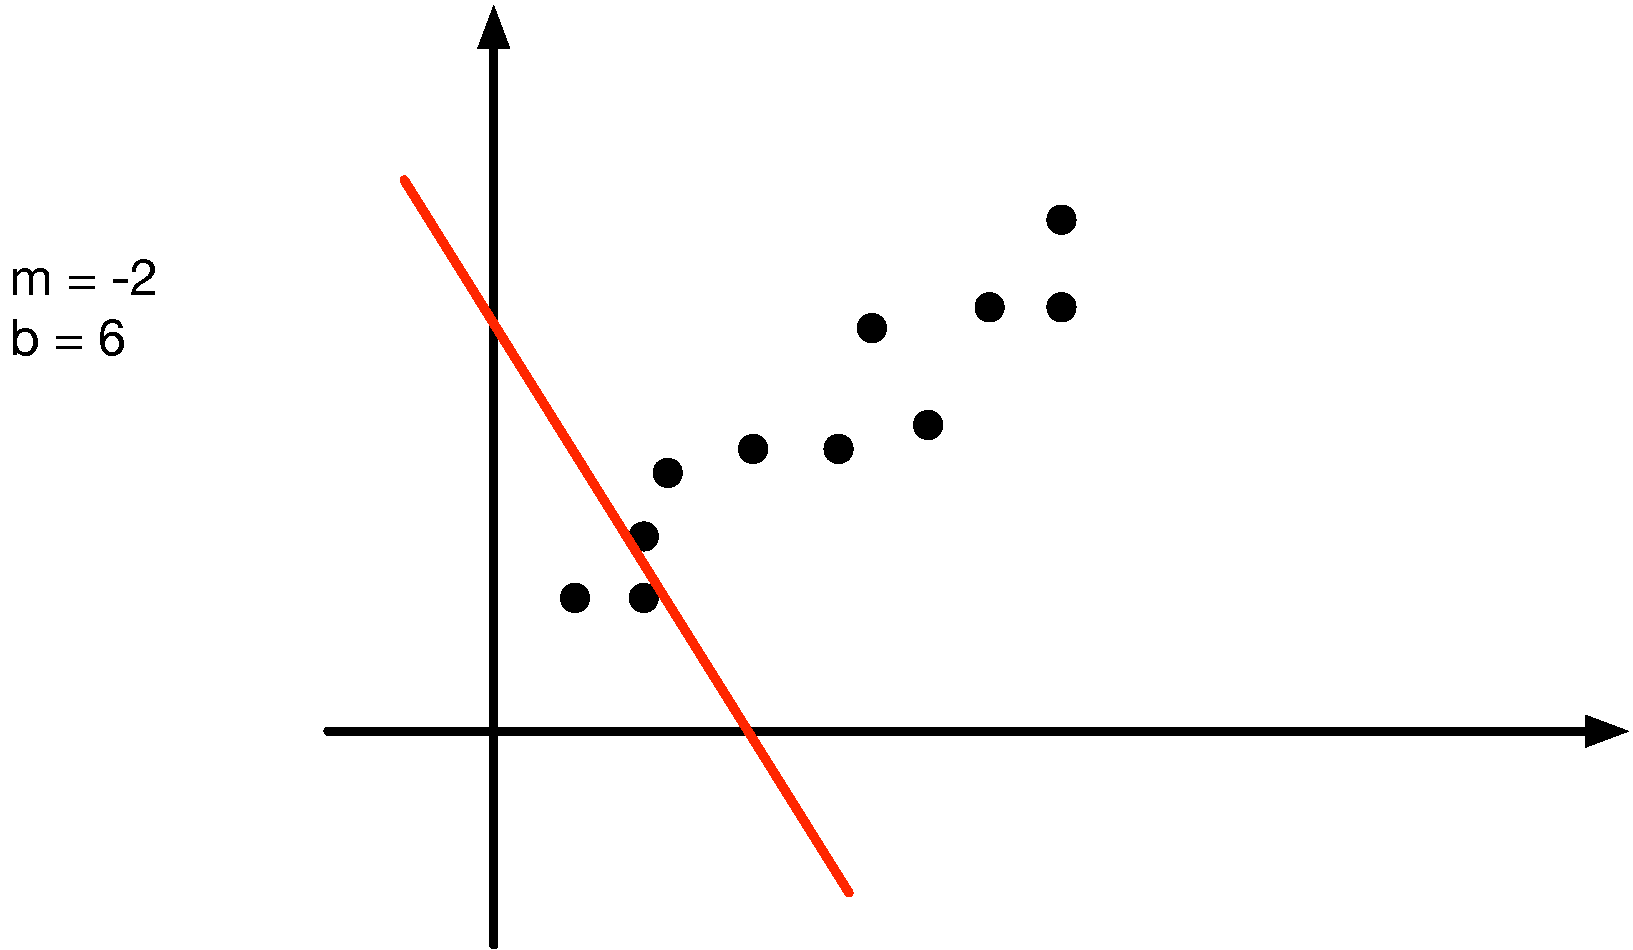
\includegraphics[width=1\textwidth]{lectGD/step1.pdf}\\
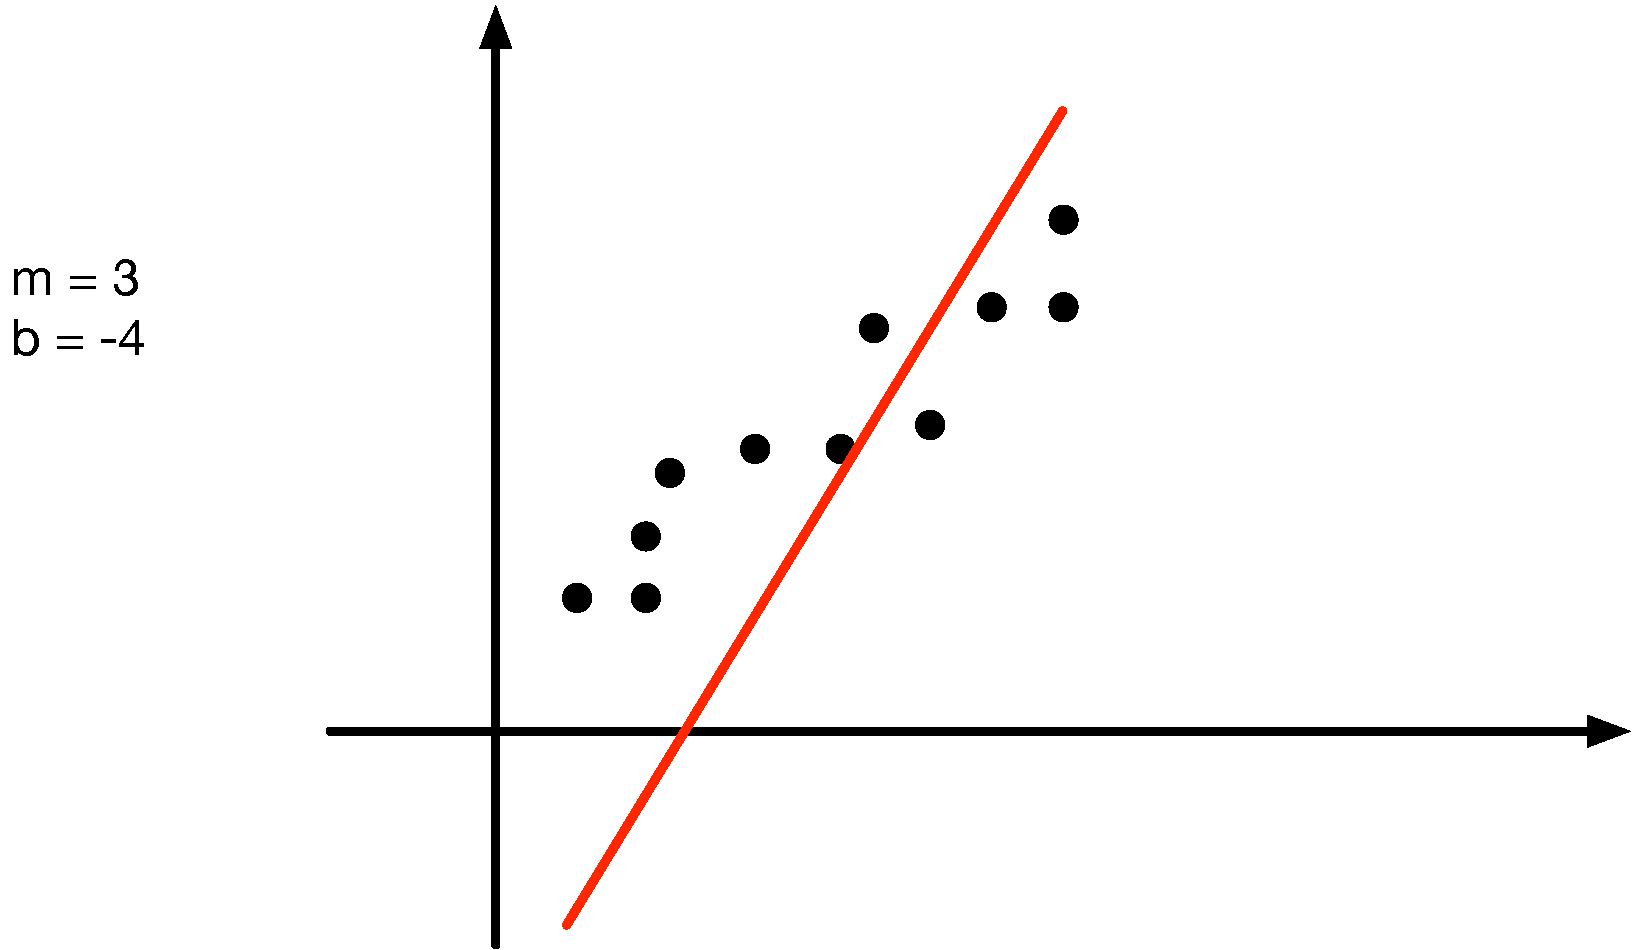
\includegraphics[width=1\textwidth]{lectGD/step2.pdf}
\end{column}
\begin{column}{0.3\textwidth}
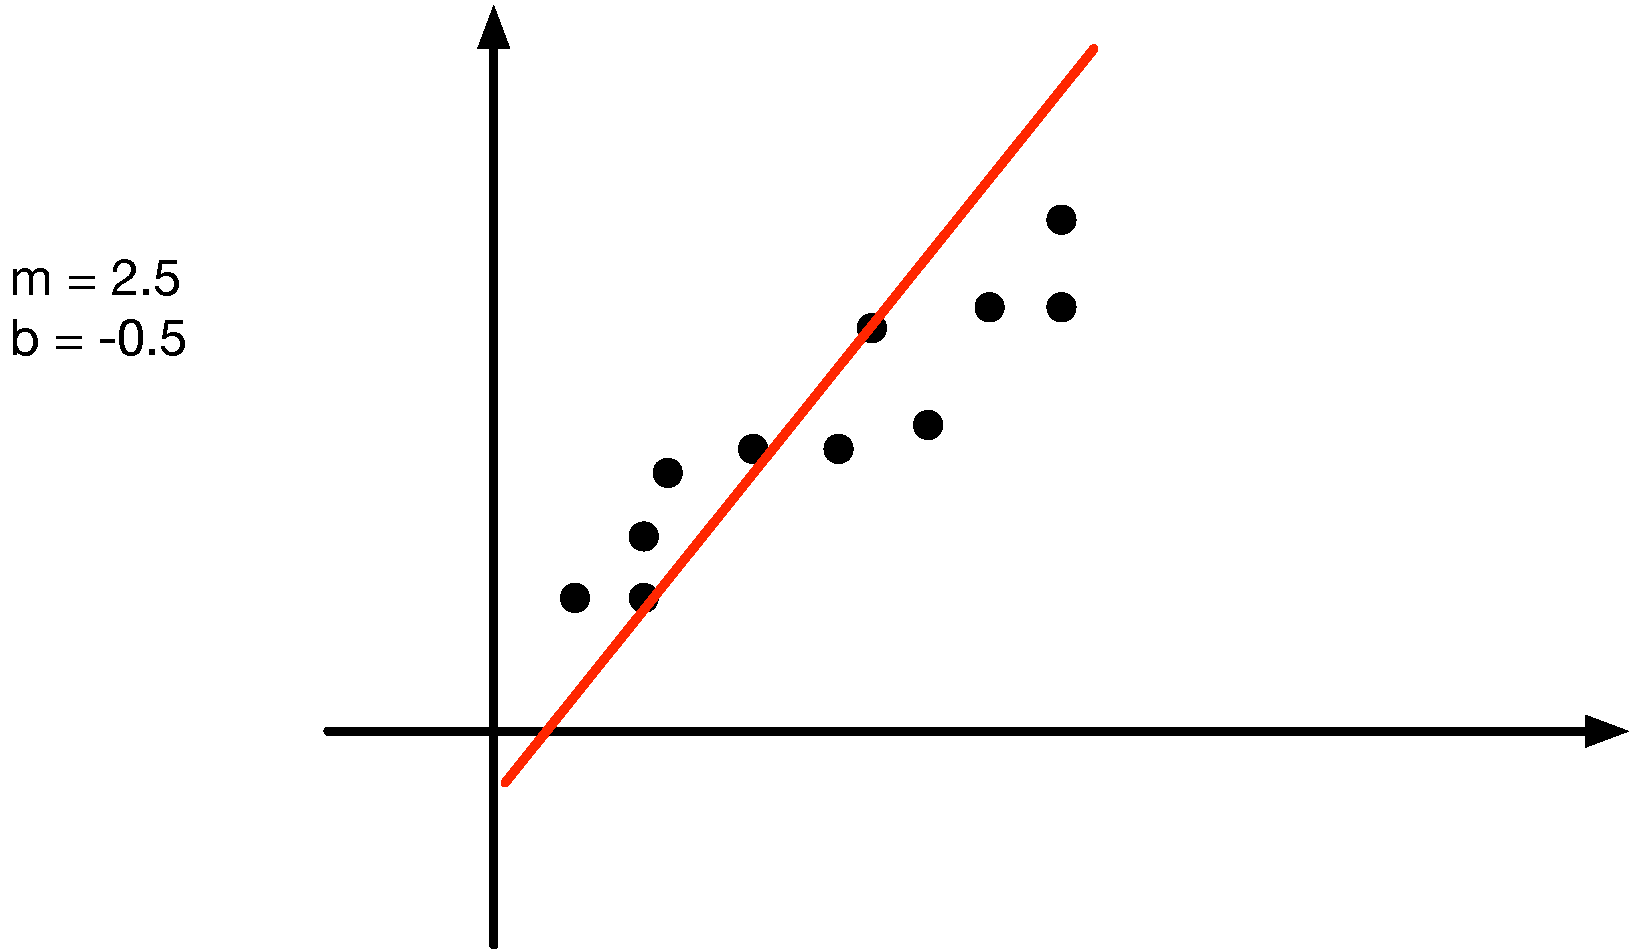
\includegraphics[width=1\textwidth]{lectGD/step3.pdf}\\
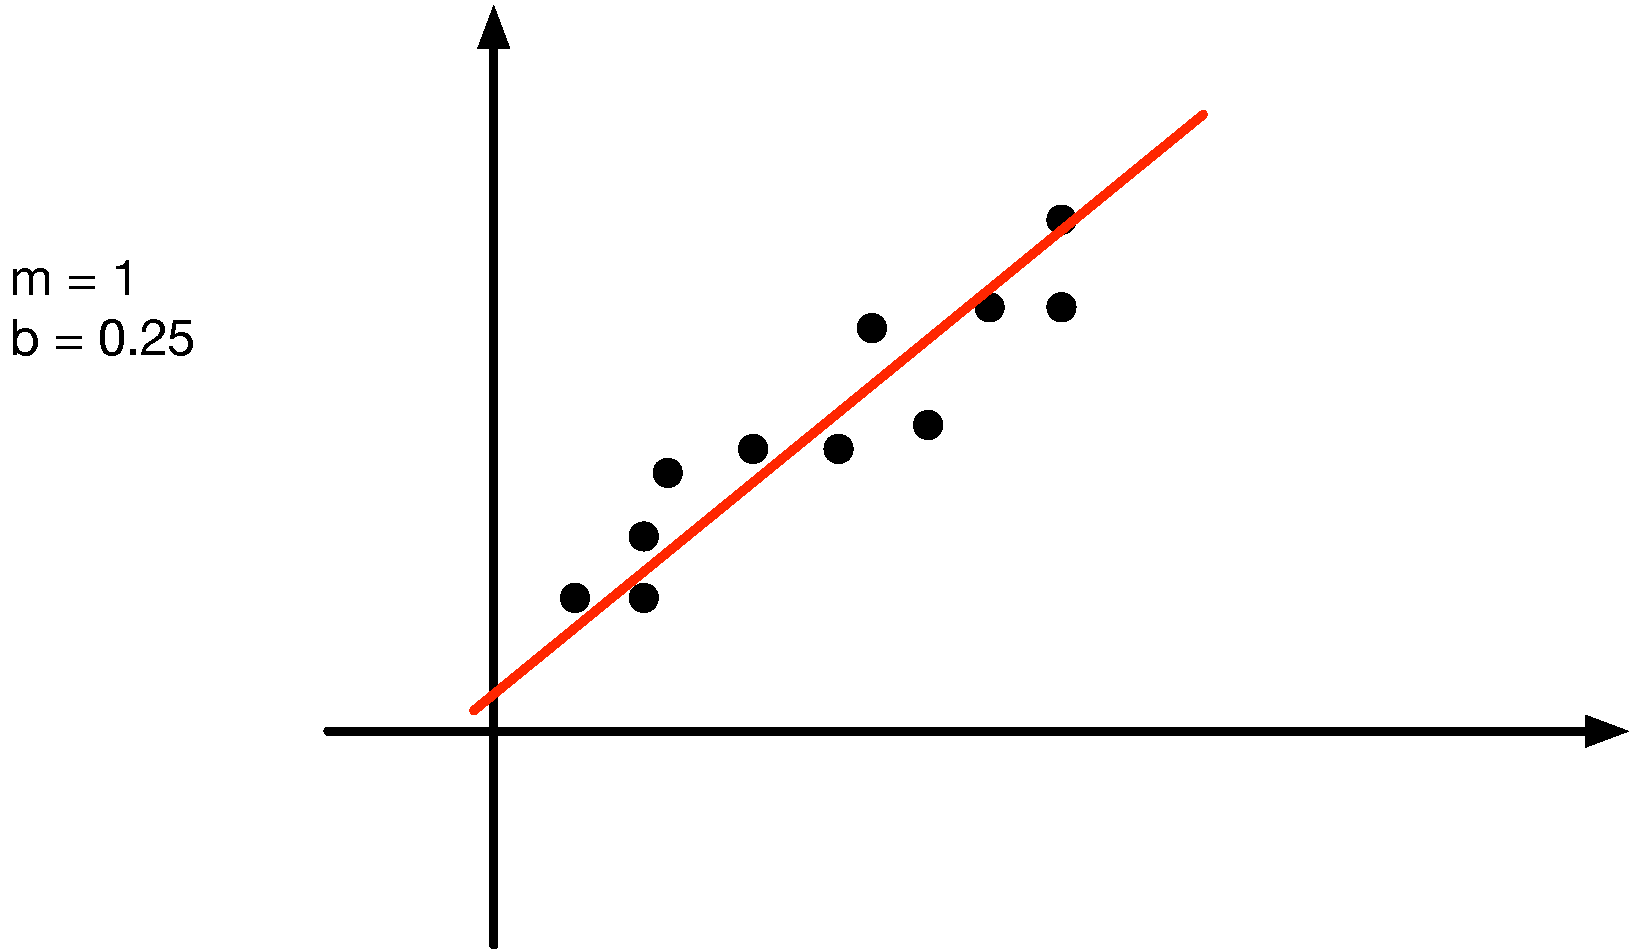
\includegraphics[width=1\textwidth]{lectGD/step4.pdf}
\end{column}
\end{columns}

\end{frame}

%***********************************************************
\begin{frame}[fragile]{The Learning Rate}

\begin{itemize}
\item How much do we change the parameter values each iteration?
\item Reconsider the algorithm:
\end{itemize}
\begin{SQL}
$\Theta_1 \leftarrow \textrm{non-stupid guess for } \Theta^*$;
$i \leftarrow 1$;
repeat {
  $\Theta_{i + 1} \leftarrow \Theta_{i} - \lambda \nabla L (\Theta_{i})$;
  $i \leftarrow i + 1$;
} while ($||\Theta_{i} - \Theta_{i - 1}||_1 > \epsilon$)
\end{SQL} 

\begin{itemize}
\item How to choose $\lambda$?
\end{itemize}

\end{frame}
%***********************************************************
\begin{frame}[fragile]{Choosing the Learning Rate: $\lambda$}

\begin{columns}[c]
\begin{column}{0.4\textwidth}
\begin{itemize}
\item Super important
	\begin{itemize}
	\item Too small: many, many passes thru the data to converge
	\item Too large: oscillate into oblivion
	\end{itemize}
\end{itemize}
\end{column}
\begin{column}{0.3\textwidth}
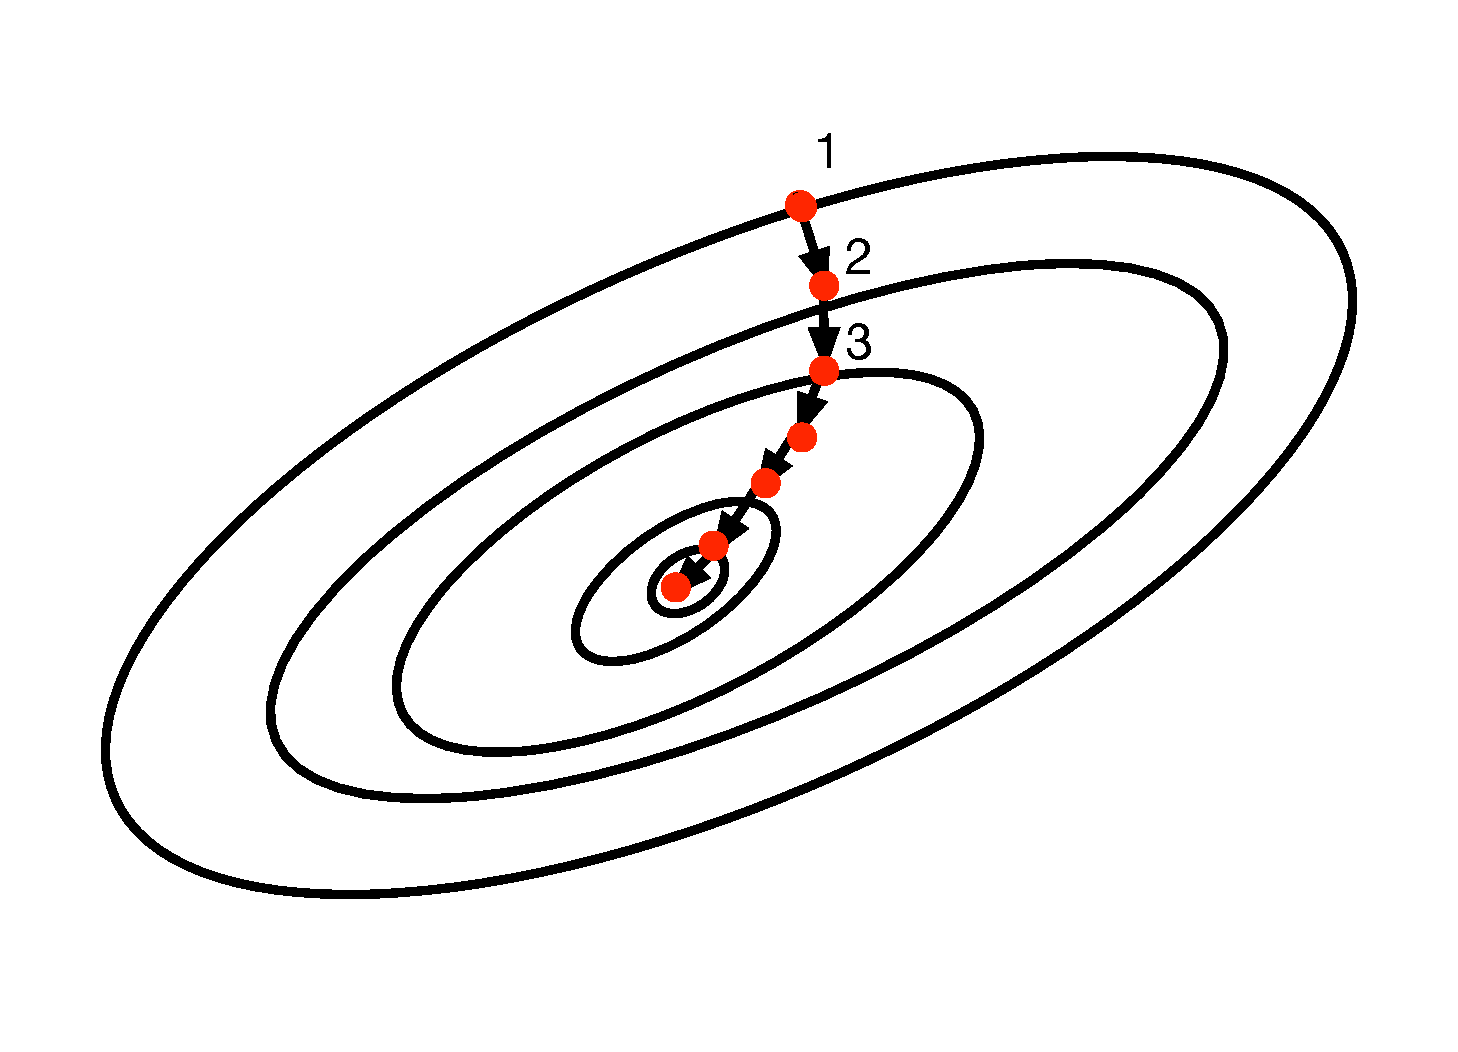
\includegraphics[width=1\textwidth]{lectGD/tooSmall.pdf}\\
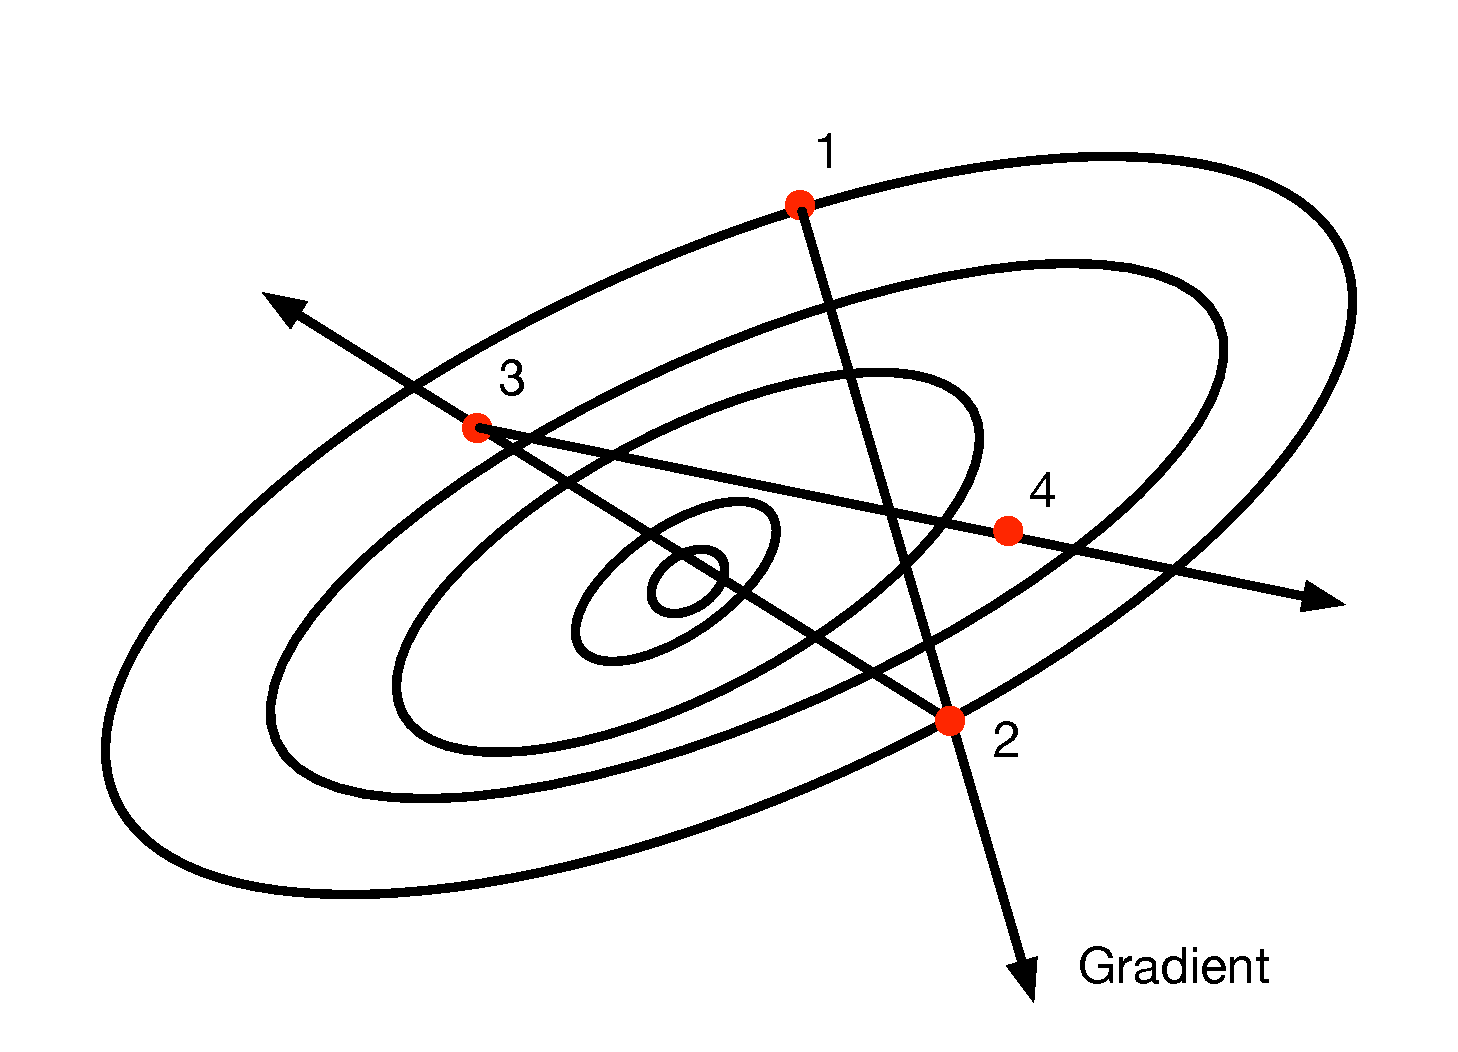
\includegraphics[width=1\textwidth]{lectGD/tooBig.pdf}\\
\end{column}
\begin{column}{0.3\textwidth}
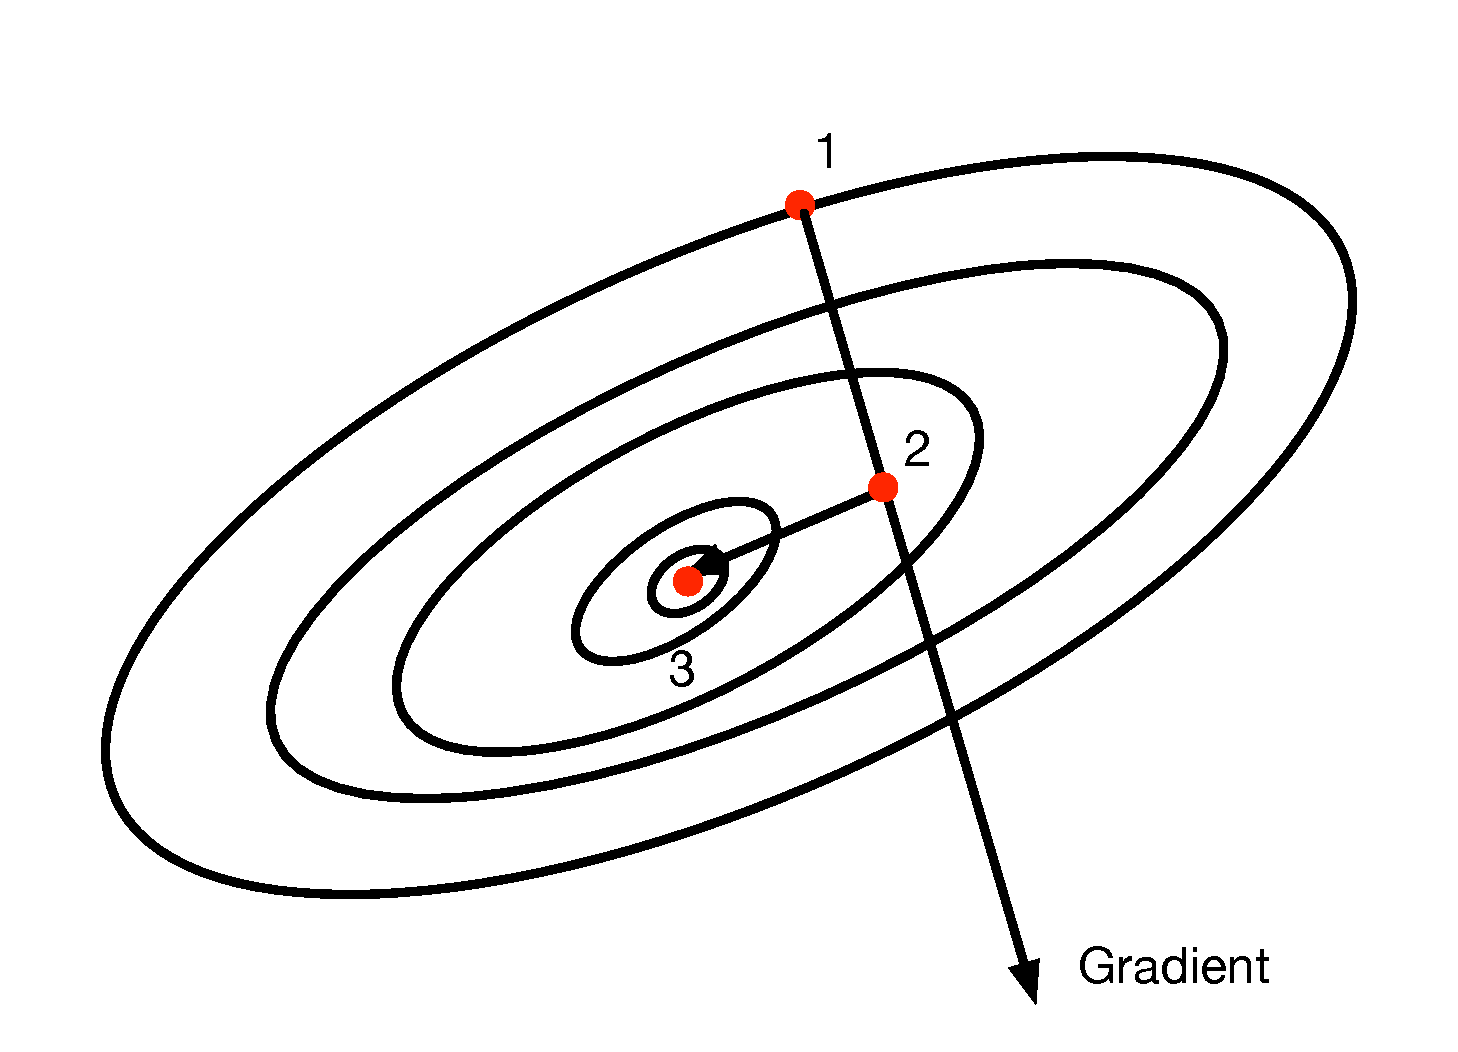
\includegraphics[width=1\textwidth]{lectGD/justRight.pdf}\\
\end{column}
\end{columns}

\end{frame}
%***********************************************************
\begin{frame}[fragile]{Choosing the Learning Rate}

\begin{itemize}
\item There are two classic approaches
\begin{enumerate}
\item Line search
\item Bold driver
\end{enumerate}
\end{itemize}

\end{frame}
%***********************************************************
\begin{frame}{Line Search}
% this is an optimization problem
\begin{itemize}
\item Best option (in terms of results) but most expensive:
	\begin{itemize}
	\item Solve another mini-optimization problem at each iteration
	\item That is, choose $\lambda$ so as to minimize $L(\Theta_{i + 1})$
	\item At lest now, it's a 1-dimensional optimization problem!
	\item Called a ``line search''
	\end{itemize}
\end{itemize}
	
\end{frame}

%***********************************************************
\begin{frame}{Line Search}

\begin{columns}[T]
\begin{column}{0.6\textwidth}
\begin{itemize}
\item Sort of like a binary search
\item But try to find a minimum, not a specific value
\item What is binary search?
\end{itemize}
\end{column}
\begin{column}{0.4\textwidth}
%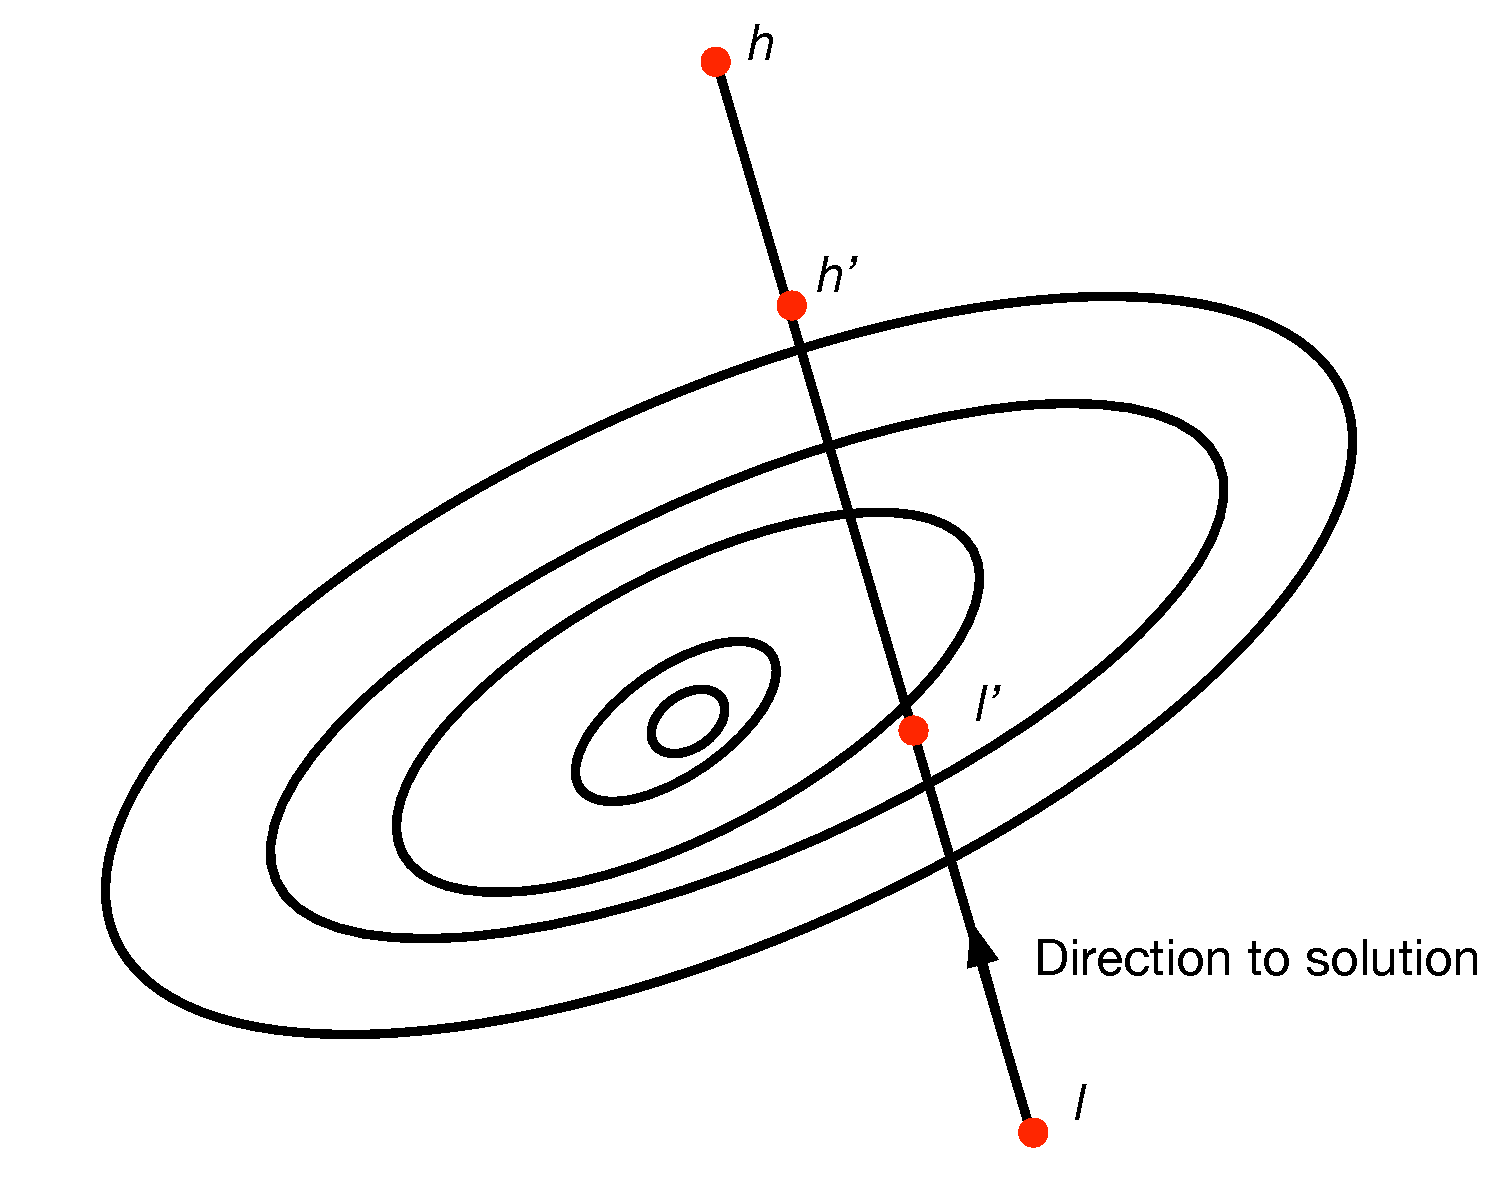
\includegraphics[width=1\textwidth]{lectGD/lineSearchHighLevel.pdf}
\end{column}
\end{columns}
	
\end{frame}

%***********************************************************
\begin{frame}{Binary Search}

\begin{itemize}
\item Also called half-interval search
\item Finds the position of a value within a sorted array
\item Say you are trying to load data into a database
\item But the load fails and gives no error
\item You want to figure out where it is failing
\item You might try to load the first half of the data 
\item If that works, the error must be in the 2nd half
\item So, try to load the first half of that data 
\item $\ldots$
\item Average performance is O(log n)
\end{itemize}

	
\end{frame}

%***********************************************************
\begin{frame}{Line Search}

\begin{columns}[T]
\begin{column}{0.6\textwidth}
\begin{itemize}
\item Sort of like a binary search
\item But try to find a minimum, not a specific value
\begin{enumerate}
\item Find the direction that minimizes the objective function
\item Decide how big of a step to take in that direction
\end{enumerate}
\begin{itemize}
\item Always have two extreme bounds $l$ and $h$ on $\lambda$
\item At each iteration, choose two $l'$, $h'$ within $[l, h]$ 
\item Breaks line segment between $l$ and $h$ three ways (two ends and a middle)
\item Evaluate loss at $l'$, $h'$
\item Cut off the worse of the two ends
	\end{itemize}
\end{itemize}
\end{column}
\begin{column}{0.4\textwidth}
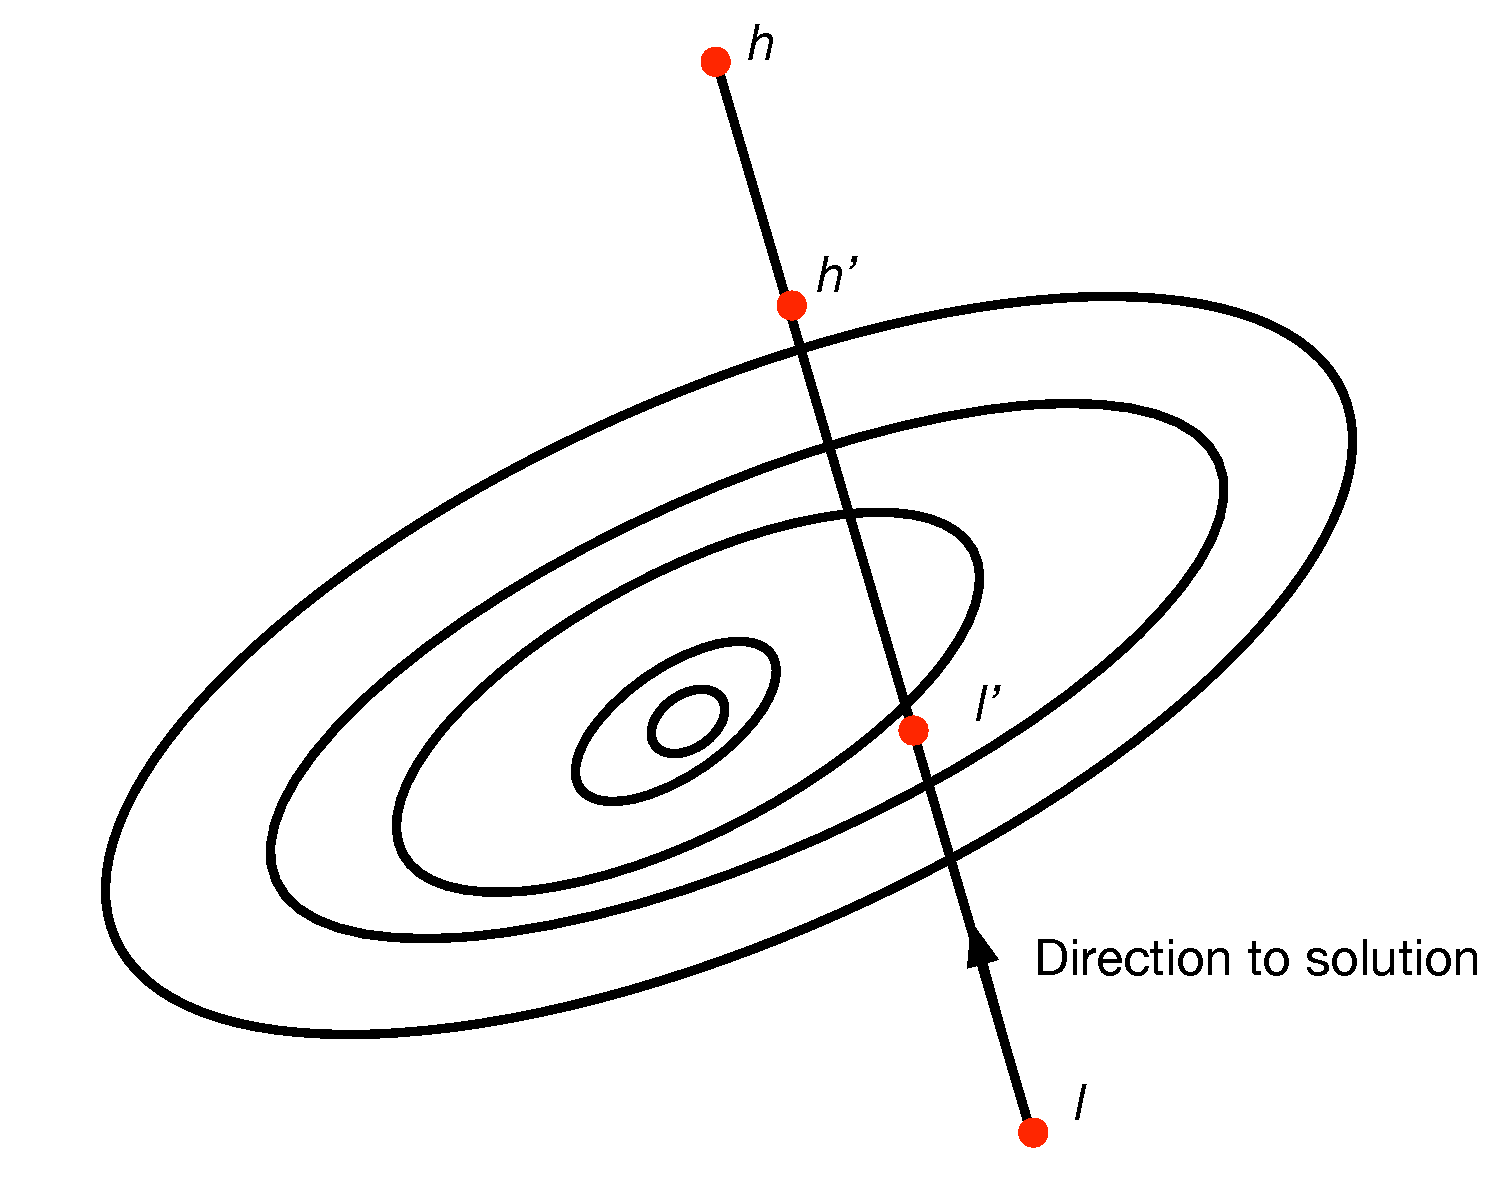
\includegraphics[width=1\textwidth]{lectGD/lineSearchHighLevel.pdf}
\end{column}
\end{columns}
	
\end{frame}

%***********************************************************
%\begin{frame}{Line Search Intuition}
%
%\begin{columns}[T]
%\begin{column}{0.5\textwidth}
%\begin{itemize}
%\item Use the gradient to give a direction
%\item Ignore the magnitude of the gradient
%	\begin{itemize}
%	\item Solve another mini-optimization problem
%	\item That is, choose $\lambda$ so as to minimize $L(\Theta_{i + 1})$
%	\item At lest now, it's a 1-dimensional optimization problem!
%	\item Called a ``line search''
%	\end{itemize}
%\end{itemize}
%\end{column}
%\begin{column}{0.5\textwidth}
%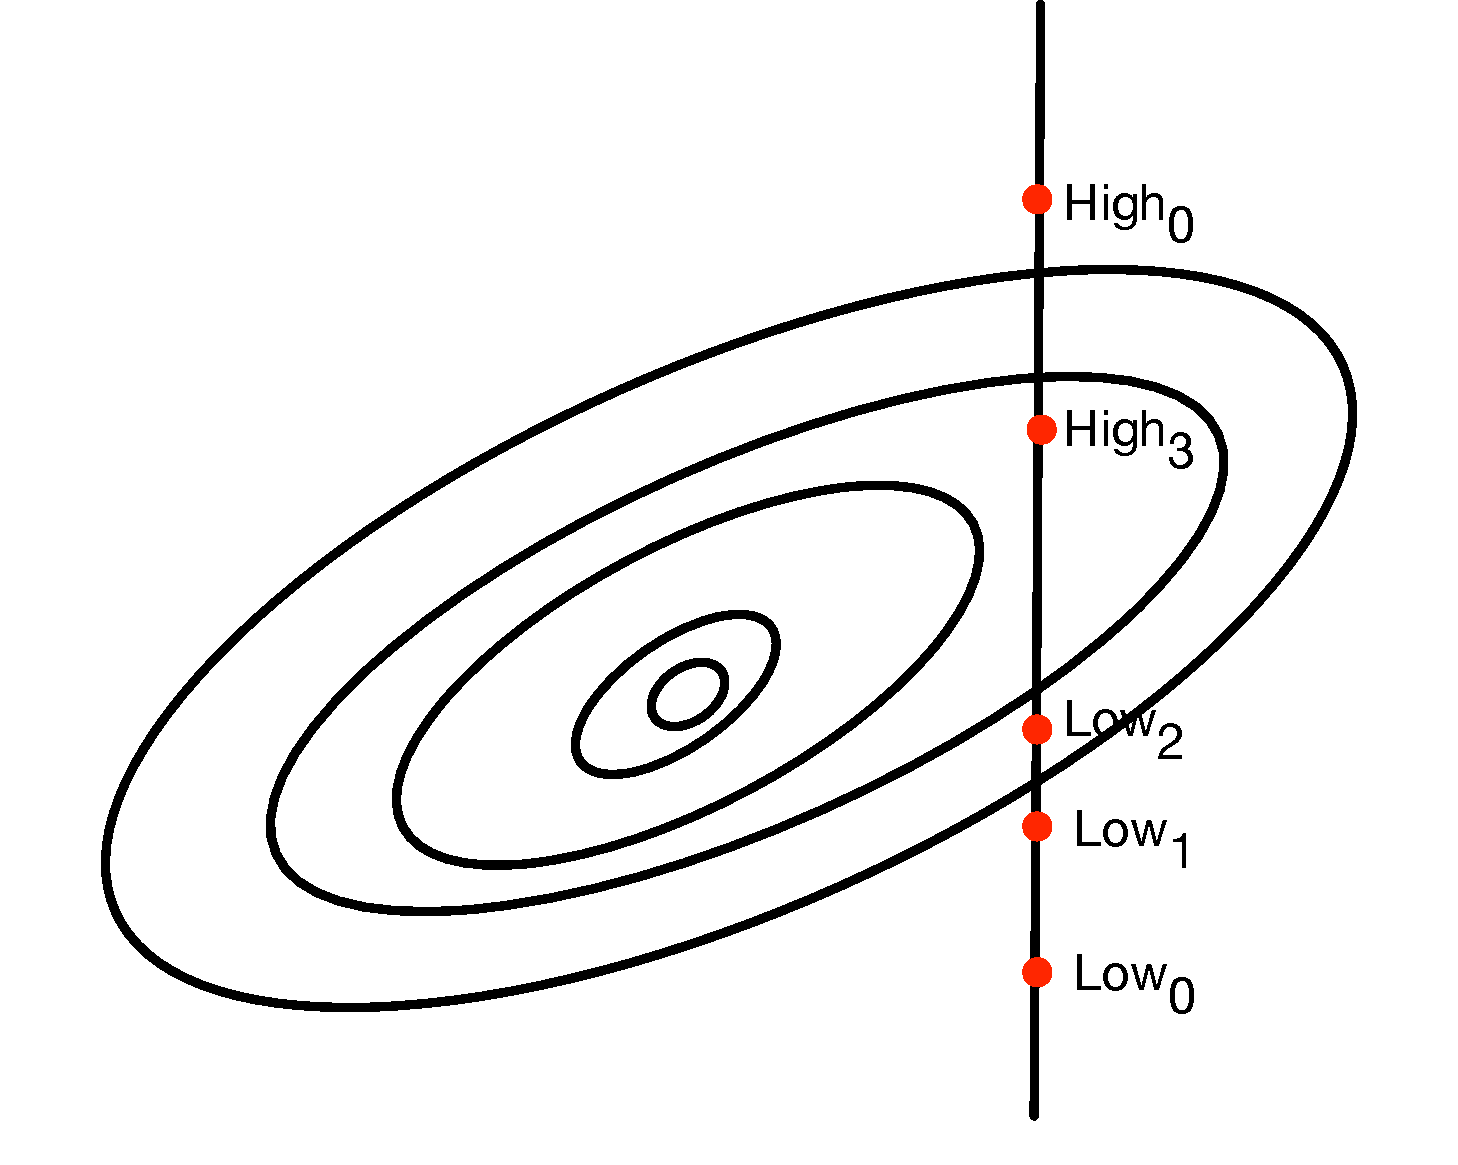
\includegraphics[width=1\textwidth]{lectGD/lineSearch1.pdf}
%\end{column}
%\end{columns}
%	
%\end{frame}
%***********************************************************
\begin{frame}[fragile]{Line Search}

\begin{columns}[T]
\begin{column}{0.5\textwidth}
\begin{SQL}
$l \leftarrow 0$;
$h \leftarrow 999999$;
while ($h - l > \epsilon$) do {
  $h' \leftarrow l + \frac{1}{c}(h - l)$;
  $l' \leftarrow h - \frac{1}{c}(h - l)$;
  loss$_h \leftarrow L (\Theta_{i} - h' \nabla L (\Theta_{i}))$;
  loss$_l \leftarrow L (\Theta_{i} - l' \nabla L (\Theta_{i}))$;
  if (loss$_h$ < loss$_l$) {
    $l \leftarrow l'$;
  else
    $h \leftarrow h'$;
  }
}
\end{SQL}
\end{column}
\begin{column}{0.5\textwidth}
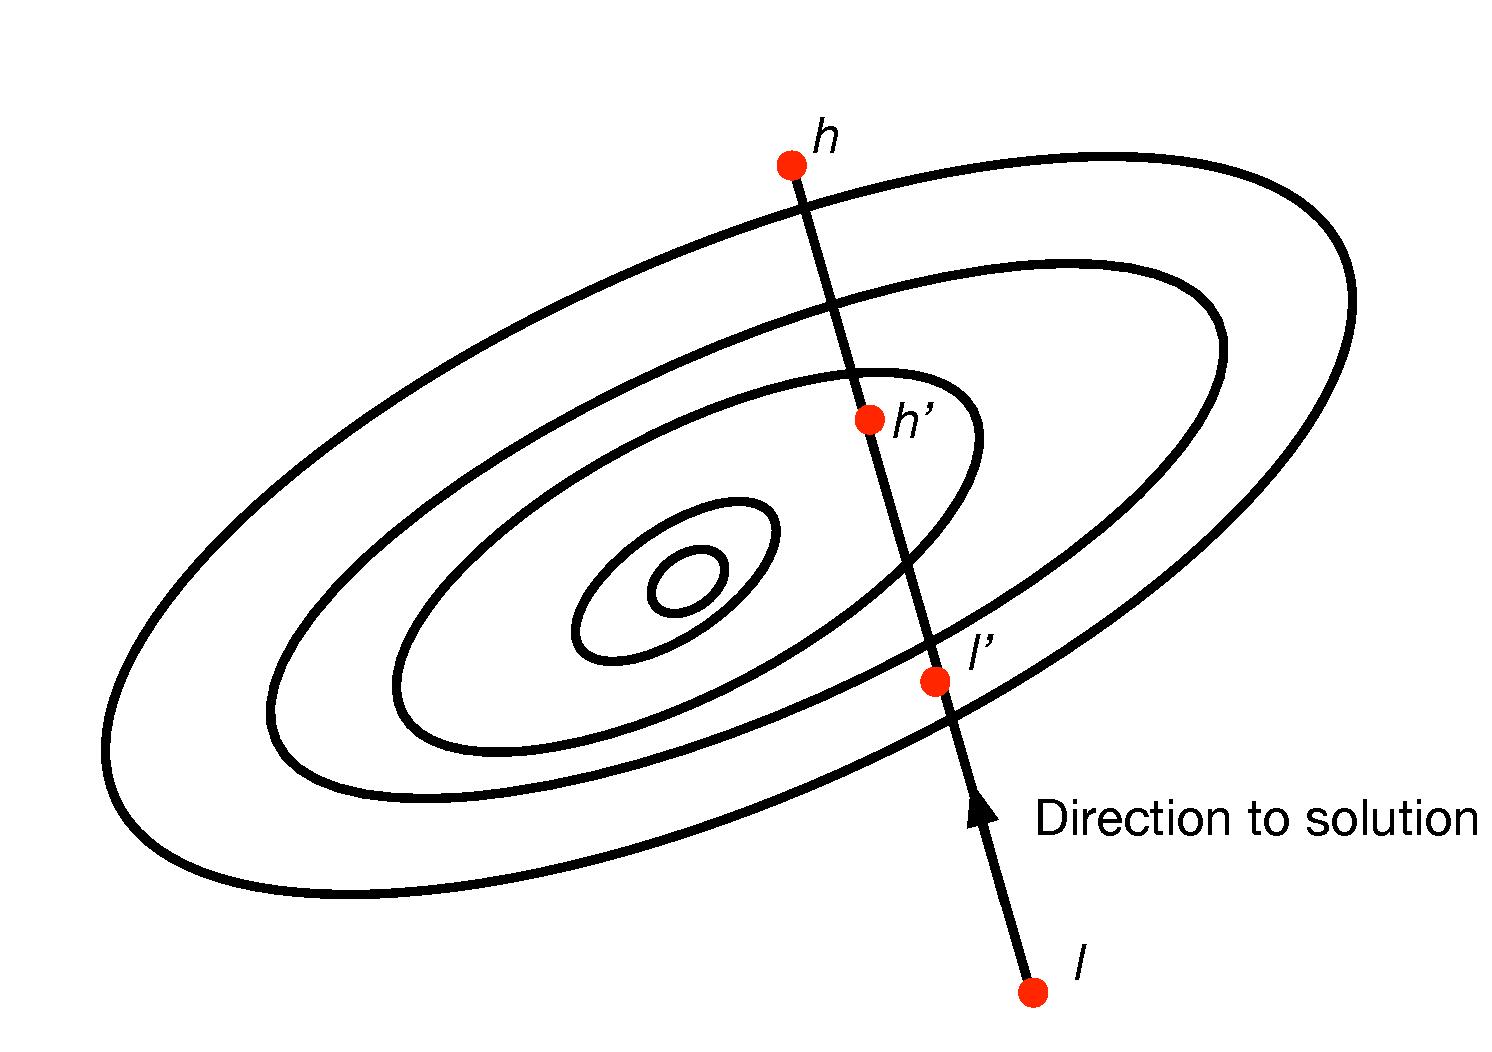
\includegraphics[width=1\textwidth]{lectGD/lineSearch2.pdf}
\end{column}
\end{columns}

\begin{itemize}
\item ``Golden section search'': $c = \frac{1}{2}(1 + \sqrt{5}) = 1.618$
\end{itemize}
	
\end{frame}
%***********************************************************
\begin{frame}{Problems with Line Search}

\begin{itemize}
\item Line search is costly!
\begin{itemize}
\item We have to keep recalculating the value of the loss function
\item This is not feasible for big data!
\end{itemize}
\end{itemize}
\end{frame}
%***********************************************************
\begin{frame}{Other Ways To Choose Learning Rate}

\begin{itemize}
\item Other standard method is ``Bold Driver''
	\begin{itemize}
	\item Widely used approach
	\end{itemize}
	\item Approach
	\begin{itemize}
	\item Make a very conservative initial guess for $\lambda$
	\item At each iteration, compute $L (\Theta_{i})$ % this can be super expensive - thousands of times more expensive than doing an iteration
	\item Better than last time?  Increment $\lambda$ just a little bit: $\lambda \leftarrow \lambda \times 1.05$
	\item Worse than last time?  Reduce $\lambda$ by a lot: $\lambda \leftarrow \lambda \times 0.5$
	\item Just one eval of loss function per iteration! 
	\end{itemize}
\end{itemize}

\end{frame}
%***********************************************************
\begin{frame}{Bold Driver Intuition}

\begin{itemize}
\item Increase $\lambda$ slowly so we don't miss a divergence
\item At first sign of a divergence, back up massively
\item Theory says that if you choose reasonable increment and decrement factors, the algorithm is guaranteed to converge
\end{itemize}

\end{frame}
%***********************************************************
%\begin{frame}{Can We do Better?}
%
%\begin{itemize} 
%\item Stochastic Gradient Descent
%\begin{itemize}
%\item 1 data point per iteration
%\item Mathematics says it's optimal in terms of convergence rate
%\end{itemize}
%\item Why does a small batch size make sense?
%\end{itemize}
%
%\end{frame}
%

%***********************************************************
\begin{frame}{Questions?}
\begin{itemize}
	\item[?] What do we know now that we didn't know before?
	\vspace{2em}
	\item[?] How can we use what we learned today?
\end{itemize}
\end{frame}

%***********************************************************
\begin{frame}{Questions?}
\begin{itemize}
	\item What do we know now that we didn't know before?
	\begin{itemize}
		\item How to solve optimization problems using Gradient Descent
		\item Different ways to decide to terminate learning
		\item Some issues with Big Data
		\item Some approaches for adapting the learning rate in Gradient Descent
	\end{itemize}
	\vspace{2em}
	\item How can we use what we learned today?
	\begin{itemize}
	\item In the next exercise!
	\end{itemize}
\end{itemize}
\end{frame}


%***********************************************************
\begin{frame}{Example}

	\begin{itemize}
	\item Prediction $f(t | b, m) = b + m \times t$
	\item Loss $L(b, m) = \sum_i \left(f(t_i | b, m) - x_i \right)^2$
	\end{itemize}
\begin{itemize}
\item First we deal with $b$ and then with $m$:
	\begin{align}
	\frac{\partial L}{\partial b} &= \frac{\partial \sum_i (f(t_i | b, m) - x_i) ^2}{\partial b} \nonumber \\
		 & = \sum_i 2(f(t_i | b, m) - x_i) \frac{\partial \left(f(t_i | b, m) - x_i \right)}{\partial b}  \nonumber \\
		&= \sum_i 2(f(t_i | b, m) - x_i) \nonumber \\
	\frac{\partial L}{\partial m} \nonumber &= \frac{\partial \sum_i (f(t_i | b, m) - x_i) ^2}{\partial m} \nonumber \\
		&= \sum_i 2(f(t_i | b, m) - x_i) \frac{\partial \left(f(t_i | b, m) - x_i \right)}{\partial m}  \nonumber \\
		&= \sum_i 2t_i(f(t_i | b, m) - x_i) \nonumber
	\end{align}
\end{itemize}

\end{frame}
\end{document}
